\documentclass[tikz,border=4pt]{standalone}
% Paleta y fuentes compartidas por el libro y las figuras (única fuente de verdad).
\RequirePackage{xcolor}
\definecolor{oxido}{HTML}{B7410E}
\definecolor{cobre}{HTML}{D27D2D}
\definecolor{carbon}{HTML}{2B2B2B}
\definecolor{azul}{HTML}{1F5F8B}
\definecolor{arena}{HTML}{F4EDE4}

\usepackage{fontspec}
\setsansfont{FiraSans}[Extension=.otf,UprightFont=*-Regular,BoldFont=*-SemiBold,ItalicFont=*-Italic,BoldItalicFont=*-SemiBoldItalic]
\setmonofont{FiraMono}[Extension=.otf,UprightFont=*-Regular,BoldFont=*-Medium,Scale=0.95]
\usetikzlibrary{positioning,arrows.meta,calc}
\begin{document}
\sffamily\small
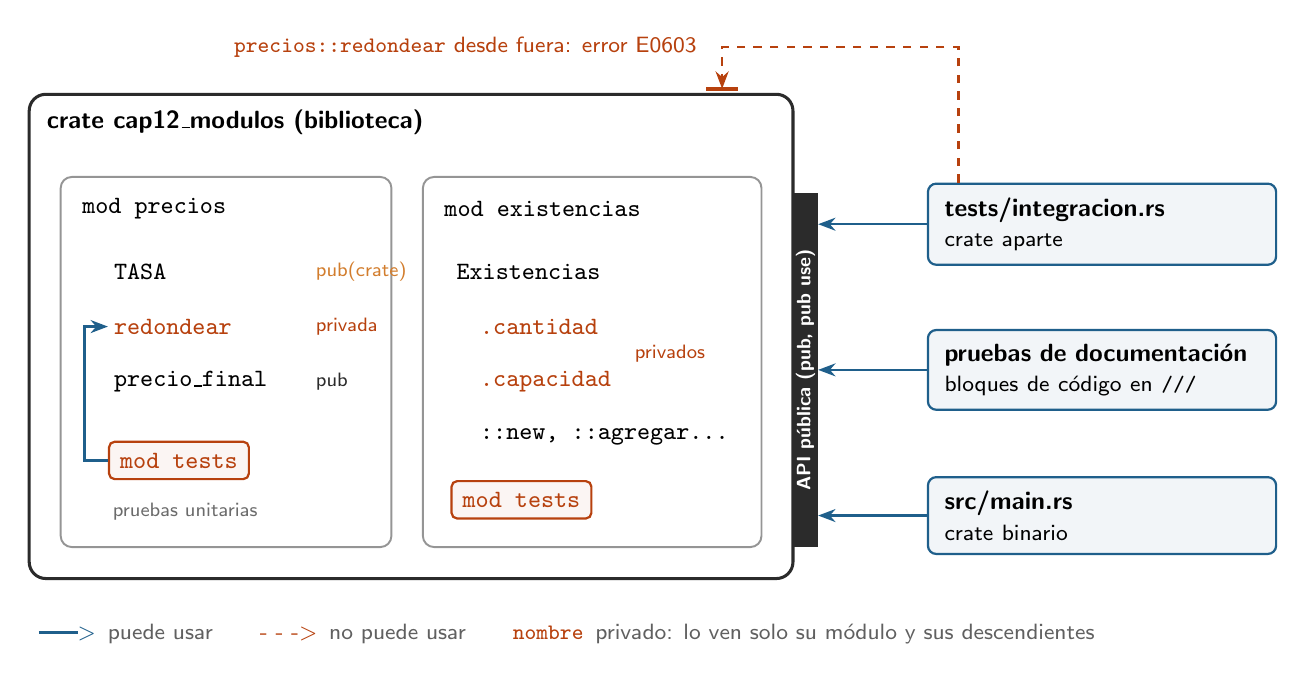
\begin{tikzpicture}[>={Stealth[length=2.2mm]},
  item/.style={font=\ttfamily\small,anchor=west,inner sep=2pt},
  etiq/.style={font=\sffamily\scriptsize,anchor=west,inner sep=1pt},
  modulo/.style={font=\ttfamily\small\bfseries,anchor=west},
  pruebas/.style={draw=oxido,line width=0.8pt,fill=oxido!5,rounded corners=2pt,
    font=\ttfamily\small,text=oxido,anchor=west,inner sep=4pt},
  externo/.style={draw=azul,line width=0.8pt,fill=azul!6,rounded corners=3pt,
    font=\sffamily\small,align=left,inner xsep=6pt,inner ysep=5pt,
    anchor=west,text width=40mm},
  ve/.style={->,azul,line width=0.9pt},
  nove/.style={->,oxido,line width=0.9pt,dashed},
  nota/.style={font=\sffamily\footnotesize,text=carbon!75,anchor=west}]
  % ----- Módulo precios -----
  \draw[carbon!50,rounded corners=4pt,line width=0.7pt]
    (0,-0.3) rectangle (4.2,-5.0);
  \node[modulo] at (0.15,-0.7) {mod precios};
  \node[item] (tasa) at (0.6,-1.5) {TASA};
  \node[etiq,text=cobre] at (3.2,-1.5) {pub(crate)};
  \node[item,text=oxido] (red) at (0.6,-2.2) {redondear};
  \node[etiq,text=oxido] at (3.2,-2.2) {privada};
  \node[item] (pf) at (0.6,-2.9) {precio\_final};
  \node[etiq,text=carbon] at (3.2,-2.9) {pub};
  \node[pruebas] (ut) at (0.6,-3.9) {mod tests};
  \node[etiq,text=carbon!70] at (0.62,-4.55) {pruebas unitarias};
  \draw[ve] (ut.west) -- ++(-0.3,0) |- (red.west);
  % ----- Módulo existencias -----
  \draw[carbon!50,rounded corners=4pt,line width=0.7pt]
    (4.6,-0.3) rectangle (8.9,-5.0);
  \node[modulo] at (4.75,-0.7) {mod existencias};
  \node[item] at (4.95,-1.5) {Existencias};
  \node[item,text=oxido] at (5.25,-2.2) {.cantidad};
  \node[item,text=oxido] at (5.25,-2.9) {.capacidad};
  \node[etiq,text=oxido] at (7.25,-2.55) {privados};
  \node[item] at (5.25,-3.6) {::new, ::agregar…};
  \node[pruebas] at (4.95,-4.4) {mod tests};
  % ----- Crate -----
  \draw[carbon,line width=1.1pt,rounded corners=6pt]
    (-0.4,0.75) rectangle (9.3,-5.4);
  \node[font=\sffamily\small\bfseries,anchor=west] at (-0.3,0.4)
    {crate cap12\_modulos (biblioteca)};
  % API pública: la frontera
  \fill[carbon] (9.3,-0.5) rectangle (9.62,-5.0);
  \node[rotate=90,font=\sffamily\scriptsize\bfseries,text=white] at (9.46,-2.75)
    {API pública (pub, pub use)};
  % ----- Crates externos -----
  \node[externo] (int) at (11.0,-0.9) {\textbf{tests/integracion.rs}\\
    \footnotesize crate aparte};
  \node[externo] (doc) at (11.0,-2.75) {\textbf{pruebas de documentación}\\
    \footnotesize bloques de código en \texttt{///}};
  \node[externo] (bin) at (11.0,-4.6) {\textbf{src/main.rs}\\
    \footnotesize crate binario};
  \draw[ve] (int.west) -- (9.62,-0.9);
  \draw[ve] (doc.west) -- (9.62,-2.75);
  \draw[ve] (bin.west) -- (9.62,-4.6);
  % Intento fallido: se detiene en el borde del crate
  \draw[nove] (int.north west) ++(0.4,0) |- (8.4,1.35) -- (8.4,0.82);
  \draw[oxido,line width=1.4pt] (8.2,0.82) -- (8.6,0.82);
  \node[nota,text=oxido,anchor=east] at (8.2,1.35)
    {\texttt{precios::redondear} desde fuera: error E0603};
  % Leyenda
  \node[nota] at (-0.4,-6.1) {\textcolor{azul}{\rule[2pt]{14pt}{1pt}\textgreater}\, puede usar\qquad
    \textcolor{oxido}{- - -\textgreater}\, no puede usar\qquad
    \textcolor{oxido}{\ttfamily nombre}\, privado: lo ven solo su módulo y sus descendientes};
\end{tikzpicture}
\end{document}
